\documentclass[conference, a4paper, 12pt]{IEEEtran}

% Package imports
\usepackage[utf8]{inputenc}
\usepackage{amsmath}
\usepackage{amsfonts}
\usepackage{amssymb}
\usepackage{graphicx, float}
\usepackage{wrapfig}
\usepackage{hyperref}
\usepackage{geometry}
\usepackage{fancyhdr}
\usepackage{titlesec}
\usepackage{listings}
\usepackage{xcolor}
\usepackage{mdframed}
\usepackage{capt-of}
\usepackage{cuted}
\usepackage{times}
\usepackage[T1]{fontenc}
\hypersetup{
    colorlinks=true,
    linkcolor=blue,
    filecolor=magenta,
    urlcolor=blue,
    }


% Space between the columns
\setlength{\columnsep}{0.45in}

% Use arabic on section
\renewcommand{\thesection}{\arabic{section}}
\renewcommand{\thesubsection}{\arabic{section}.\arabic{subsection}}
\renewcommand{\thesubsubsection}{\thesubsection.\arabic{subsubsection}}

% Page layout
\geometry{margin=0.75in}
\pagestyle{fancy}
\fancyhf{}
\fancyhead[L]{\leftmark}
\fancyhead[R]{\thepage}
\graphicspath{{images/}}
% Title format
\titleformat{\section}
  {\normalfont\Large\bfseries}{\thesection}{1em}{}
\titleformat{\subsection}
  {\normalfont\large\bfseries}{\thesubsection}{1em}{}
\titleformat{\subsubsection}
  {\normalfont\normalsize\bfseries}{\thesubsubsection}{1em}{}
\renewenvironment{abstract}
 {\small\quotation
  \noindent\textbf{Abstrato:}\medskip\par}
 {\medskip\endquotation}
\titleformat{\paragraph}
  {\normalfont\normalsize\bfseries}{\theparagraph}{1em}{}
\titlespacing*{\paragraph}
  {0pt}{3.25ex plus 1ex minus .2ex}{1.5ex plus .2ex}
% Code listing settings
\lstset{
    language=Python,
    basicstyle=\ttfamily\footnotesize,
    keywordstyle=\color{blue},
    stringstyle=\color{red},
    commentstyle=\color{green},
    showstringspaces=false,
    numbers=left,
    numberstyle=\tiny,
    stepnumber=1,
    numbersep=5pt,
    frame=single,
    breaklines=true,
    breakatwhitespace=false,
    tabsize=4,
    captionpos=b,
}

% Title and author
\title{Desenvolvimento da Aplicação Flask}
\author{
    \IEEEauthorblockN{Lucas Puhl Gasperin, }
    \and
    \IEEEauthorblockN{Renan Pamplona, }
    \and
    \IEEEauthorblockN{Renan Czervinski, }
    \and
    \IEEEauthorblockN{Tiago Follador, }
}
\date{}

\begin{document}
\maketitle
\begin{strip}
  \vspace{5pt}
\par\noindent\rule{\textwidth}{1pt}
  \vspace{10pt}
  \begin{abstract}
  Neste documento, apresentamos uma descrição detalhada do desenvolvimento do Gasperin Web Services, uma aplicação inovadora que utiliza o framework Flask para proporcionar aos postos de saúde públicos um meio eficiente de gerenciar o fluxo de pessoas dentro de suas instalações, ao mesmo tempo que monitora as condições climáticas internas.

  O desenvolvimento de um projeto direcionado aos postos de saúde representa um desafio significativo, dada a importância crítica desses serviços para milhões de brasileiros. Qualquer melhoria na infraestrutura pode ter um impacto direto na qualidade do atendimento e na eficiência operacional. No entanto, a infraestrutura atual frequentemente se mostra obsoleta e incapaz de acompanhar as demandas crescentes. A falta de investimento adequado por parte do governo também limita severamente as oportunidades de inovação neste setor vital.

  O objetivo principal deste documento é explorar como enfrentamos um dos desafios mais ocorrentes enfrentados pelos postos de saúde através da aplicação de recursos da ciência da computação. Além de discutir a implementação prática do "Gasperin Web Services", também abordamos as potenciais melhorias e expansões que podem ser incorporadas no futuro. Isso inclui não apenas aprimorar a capacidade de gerenciamento de fluxo de pacientes, mas também explorar novas funcionalidades que poderiam melhorar significativamente a experiência tanto para pacientes quanto para profissionais de saúde.
  \end{abstract}

\vspace{10pt}
\par\noindent\rule{\textwidth}{1pt}

\end{strip}

\section{Introdução}
  Nos bastidores da saúde pública, os postos de saúde desempenham um papel fundamental na oferta de cuidados acessíveis e eficazes à população brasileira. No entanto, a gestão eficiente desses estabelecimentos enfrenta desafios constantes, desde o controle preciso do fluxo de pacientes até o gerenciamento das condições ambientais internas. Em resposta a essas necessidades críticas, surge a $Gasperin$ $Web$ $Services$, uma inovadora aplicação desenvolvida sobre o framework Flask, projetada para revolucionar como os postos de saúde monitoram e otimizam suas operações diárias.

  Nós criamos uma aplicação que não apenas monitora em tempo real a ocupação dos espaços físicos, ajustando automaticamente a climatização conforme a demanda, mas também visa resolver um dos desafios mais persistentes enfrentados pelos postos de saúde públicos brasileiros. A combinação de tecnologia avançada com princípios de gestão eficiente permite não apenas melhorar o conforto dos pacientes e funcionários, mas também contribuir significativamente para a redução do consumo energético e a sustentabilidade ambiental.

  Desenvolver um projeto voltado para um setor tão crucial como a saúde pública não é tarefa simples. Cada decisão tomada durante o desenvolvimento do "Gasperin Web Services" visa não apenas otimizar a operação diária dos postos de saúde, mas também garantir que cada ajuste tecnológico seja um passo em direção a um atendimento mais eficiente e equitativo para todos os usuários do sistema de saúde pública.

  Durante seu desenvolvimento, buscamos criar uma aplicação que não apenas oferecesse uma solução ao problema, mas também a possibilidade de ampliar ainda mais seus recursos, a fim de, possivelmente, fornecer soluções a problemas ainda maiores. Isso inclui discutir como o "Gasperin Web Services" pode ser adaptado para enfrentar desafios futuros e oportunidades de expansão, promovendo uma melhoria contínua na entrega de serviços de saúde pública no Brasil.

  Em resumo, a $Gasperin$ $Web$ $Services$ não é apenas uma solução tecnológica; é um compromisso com a inovação e a qualidade no setor de saúde pública. Ao integrar avanços da ciência da computação com as necessidades urgentes do atendimento médico, esperamos não apenas melhorar as operações dos postos de saúde, mas também estabelecer um padrão de excelência que inspire futuras iniciativas de saúde digital em todo o país.

  \section{Objetivos}
  \subsection{Objetivo Geral}
  O objetivo é criar uma aplicação que combine recursos de software e hardware visando inovar os postos de saúde públicos a fim de um controle de fluxo de pessoas e um monitoramento de temperatura ambiente optimizados. Para tal, utilizaremos o framework Flask em conjunto com um banco de dados relacionalMySQL, bem como um dispositivo IOT via protocolo MQTT. Ademais, combinaremos tecnologias de front e back-end para criar uma aplicação interativa, dinâmica e de simples uso.

  \subsection{Objetivos Específicos}
\begin{itemize}
  \item Construir protótipos em
EPP com sensores e atuadores.
\item Codificar sistemas web
utilizando conceitos de
arquitetura de software, por meio
de requisições e respostas aos
serviços síncronos e assíncronos.
\item Construir bancos de dados
com os requisitos de dados da
aplicação e realizar a integração
com o sistema web utilizando
framework de Mapeamento
Objeto Relacional (ORM – Object
Relational Mapper).
\item Realizar a integração de
sistemas web, projetos de banco
de dados e microcontroladores
utilizando interfaces de
comunicação para solucionar
demandas da IoT.
\end{itemize}

\section{Metodologia}
\label{sec:metodologia}
Este projeto foi desenvolvido utilizando o $framework$ $Flask$, e seguindo a arquitetura $Model-View-Controller$ (MVC), em conjunto com diversas tecnologias de $front$ e $back-end$. Além do fato de que foi requisitado, esta escolha providencia uma aplicação web robusta, escalável e de fácil manutenção.

\subsection{Camadas da Aplicação}
\begin{itemize}
  \item A camada $Model$ é responsável pelo gerenciamento dos dados, utilizando o banco de dados $MySQL$.

  \item A camada $View$ se refere aos $templates$ $html$ da aplicação.

  \item A camada $Controllers$ gerencia as rotas da aplicação.
\end{itemize}

\subsection{Hardware}
Utilizamos uma ESP32 para gerenciar os equipamentos e enviar dados via Wi-Fi. Os componentes principais incluem um sensor de temperatura (DHT22) e um leitor de tags para detectar a passagem de pessoas. Dois servomotores controlam a abertura e fechamento de portas e janelas, agilizando o serviço e prevenindo a propagação de doenças. A comunicação entre o hardware e o software é realizada via protocolo MQTT, garantindo a transmissão eficiente de dados.

\begin{figure}[h]
  \begin{center}
    
\includegraphics[width=0.30\textwidth]{schizo.jpeg}
  \end{center}
\end{figure}

\subsection{Banco de Dados}
Para o armazenamento dos dados, optamos pelo $MySQL$, um sistema de gerenciamento de banco de dados relacional ($RDBMS$) utilizado devido à sua eficiência e confiabilidade. O banco de dados foi projetado para suportar as operações necessárias da aplicação. A conexão com o banco de dados é feita através da biblioteca $PyMySQL$ e as interações através da biblioteca $SQLAlchemy$.

$EXPLICAR A INTERAÇAO, FUNCS E OS CARAIO A 4$

\subsection{Front-End}
O $front-end$ da aplicação foi desenvolvido utilizando $HTML$ e $Jinja2$ para os $templates$, permitindo a renderização dinâmica das páginas web. Além disso, utilizamos $CSS$ para estilização e $JavaScript$ para adicionar interatividade e efeitos visuais. Essa combinação de tecnologias $front-end$ garantiu uma interface de usuário responsiva e intuitiva.

\subsection{Implementação}
A implementação seguiu uma abordagem iterativa e incremental, com revisões e melhorias contínuas ao longo do processo de desenvolvimento. O uso do Flask, juntamente com o MySQL, CSS, JavaScript, HTML e Jinja2, proporcionou uma base sólida para a criação de uma aplicação eficiente e funcional, atendendo aos objetivos propostos de controle de fluxo e conforto nos postos de saúde públicos.

\subsection{Configuração do Projeto}
A aplicação utiliza diversas tecnologias, e para suas instalações localmente, é recomendado acessar o \href{https://github.com/Lucas-LPG/gws}{Repositório Oficial} do projeto e seguir os passos abaixo.


\begin{lstlisting}[language=bash, caption=Project Setup]

# Clone o repositorio
git clone https://github.com/Lucas-LPG/gws

# Instale os requisitos
pip install -r requirements.txt

\end{lstlisting}

\subsection{Estrutura da Aplicação}
O projeto possui 6 diretórios relevantes: $ESP32$, $controllers$, $db$, $models$, $static$ e $views$. A estrutura de diretórios da aplicação como um todo é a seguinte:


\begin{lstlisting}[caption=Estrutura dos Diretórios]

.
    /ESP32
    /__pycache
    /controllers
        /__pycache__
    /db
        /__pycache__
    /models
        /__pycache__
    /static
        /css
        /img
        /js
    /views
        /actuators
        /devices
        /historic
        /kits
        /layouts
        /sensors
        /users

\end{lstlisting}

Além daqueles já listados acima - pertencentes a arquitetura $MVC$, o diretório $ESP32$ contém os arquivos necessários para lidar com a conexão entre a aplicação e o dispositivo $IOT$, via protocolo $MQTT$. O diretório $db$ lida com todas as operações necessárias para iniciar o banco de dados da aplicação, o que significa estabelecer a conexão, criar o usuário e as tablas, gerenciar os $triggers$ e executar a inserção inicial. Por fim, o diretório $static$ lida com os elementos estáticos da aplicação, portanto arquivos $css$, $JavaScript$ e imagens.

\subsubsection{Models}
O diretório models contém todas as classes que representam os objetos a serem persistidos no banco de dados, juntamente com seus respectivos métodos. As classes incluídas são: Actuators, Devices, Historic, Kits, Sensors e Users. Cada uma dessas classes está relacionada a uma tabela específica do banco de dados e define os atributos e métodos necessários para manipulação dos dados.

\paragraph{Users}
A classe Users é responsável por armazenar e gerir as informações sobre os usuários. A classe armazena dados como nome, senha e o cargo que o usuário exerce.

Os atributos da classe são:
\begin{itemize}
  \item $id$: Utilizado para identificar cada usuário de maneira rápida e eficiente, sendo um número único.
  \item $name$: Nome do usuário em questão, deve ser um nome único e não pode ser nulo.
  \item $password$: Senha do usuário para realizar o login de maneira segura, não pode ser nula.
  \item $role$: O cargo que o usuário está exercendo no gerenciamento dos dados, sendo esses cargos limitados a admin, estatístico e operador.
\end{itemize}

Os métodos da classe são, em geral, para realizar busca, validação, inserção, atualização e remoção dos usuários.

\begin{itemize}
  \item $validate\_user$: Valida o usuário com base no nome e senha passados como parâmetros. Realiza uma busca e verifica se esses parâmetros estão contidos no banco de dados.
    \item $insert\_into\_users$: Realiza a inserção de um novo usuário no banco de dados, passando seu nome, senha e cargo como parâmetros.
    \item $select\_all\_information\_from\_users$: Busca e mostra todas as informações sobre todos os usuários presentes no banco de dados. As informações de retorno são nome de usuário, cargo, ID de usuário e nome do kit.
    \item $select\_all\_from\_users$: Retorna todas as informações dos objetos presentes na classe Users, como seus IDs, nomes, senhas e cargos.
    \item $select\_from\_users$: Realiza uma busca com base na condição passada como parâmetro (por exemplo, um ID de usuário específico) e retorna o usuário, se existir.
    \item $select\_user\_by\_id$: Retorna o usuário com ID igual ao passado como parâmetro na função, caso exista.
      \item $select\_user\_by\_name$(name): Retorna o usuário com nome igual ao passado como parâmetro na função, caso exista.
      \item $update\_given\_user$: Realiza a atualização dos dados de um usuário específico com os novos dados passados como parâmetros (ID de usuário, nome de usuário, senha do usuário e cargo).
      \item $delete\_user\_by\_id$: Realiza a remoção de um usuário com base no ID dele, passado como parâmetro.
\end{itemize}


\paragraph{Kits}
A classe Kit armazena os dados dos kits, que sao os nomes dos kits e o id do usuario que tem acesso a ele.

Os atributos da classe são:
\begin{itemize}
  \item $id$: Utilizado para identificar cada kit de maneira rápida e eficiente, sendo um número único e autoincrementado.
  \item $name$: Nome do kit em questão, deve ser um nome único e não pode ser nulo.
  \item $user\_id$: Utiliza o ID do usuário para identificar qual usuário tem acesso a esse kit.
\end{itemize}

Os métodos da classe são, em geral, para realizar busca, inserção, atualização e remoção dos kit.

\begin{itemize}
  \item $select\_all\_from\_kits$: Seleciona todas as informações sobre os kits, incluindo o ID do kit, seu nome, o nome do usuário que possui o kit, o total de sensores e o total de atuadores.
    \item $select\_kit\_by\_id$: Realiza uma busca e seleciona o kit que tenha o ID igual ao passado como parâmetro.
    \item $select\_kit\_by\_name$:  Realiza uma busca e seleciona o kit que tenha o nome igual ao passado como parâmetro.
    \item $update\_given\_kit$: Atualiza o nome e o ID do usuário de um kit específico, identificado pelo seu ID. Todas as informações necessárias para a atualização, como o novo nome do kit e o novo ID do usuário, são passadas como parâmetros.
    \item  $delete\_kit\_by\_id$: Remove o kit que possui o ID igual ao passado como parâmetro.
\end{itemize}

\paragraph{Devices}
A classe Device armazena os dados dos dispositivos utilizados pelos kits, como seu ID, nome, valor e o ID do kit ao qual pertence.

Os atributos da classe são:
\begin{itemize}
  \item $id$: Utilizado para identificar cada dispositivo de maneira rápida e eficiente, sendo um número único e autoincrementado.
  \item $name$: Nome do dispositivo em questão, não pode ser nulo.
  \item $value$: Armazena o valor do dispositivo em questao.
  \item $kit\_id$: Armazena o ID do kit ao qual o dispositivo pertence.
\end{itemize}

Os métodos da classe são para realizar buscas especificas, com base no id e no nome.

\begin{itemize}
  \item $select\_device\_by\_name$: Realiza uma busca e seleciona o dispositivo com base no nome, que é passado como parâmetro.
    \item $select\_device\_by\_id$: Realiza uma busca e seleciona o dispositivo com o ID igual ao passado como parâmetro.
\end{itemize}

\paragraph{Actuators}
A classe Actuator armazena os dados dos atuadores, incluindo o seu ID, tópico para receber informações e o ID do dispositivo ao qual está associado.

Os atributos da classe são:
\begin{itemize}
  \item $id$: Utilizado para identificar cada atuador de maneira rápida e eficiente, sendo um número único e autoincrementado.
  \item $topic$: Armazena o tópico através do qual o atuador se comunica com o servidor via MQTT. Não pode ser nulo.
  \item $device\_id$:  Armazena o ID do dispositivo ao qual o atuador pertence.
\end{itemize}

Os métodos da classe são, em geral, para realizar busca, inserção, atualização e remoção dos atuadores.

\begin{itemize}
  \item $insert\_actuator$: Realiza a inserção de um novo atuador, utilizando como parâmetros o nome do kit, o ID do kit, o nome do dispositivo, o valor e o tópico. Se o dispositivo já existir, associa o atuador a ele; caso contrário, cria um novo dispositivo e associa o atuador a ele.
  \item $select\_all\_from\_actuators$: Realiza uma busca e retorna todas as informações sobre os atuadores, incluindo o tópico, o ID dos atuadores, o ID do dispositivo, o nome do dispositivo, o valor do dispositivo e o nome do kit.
  \item $update\_given\_actuator$: Realiza a atualização do atuador com base no ID do dispositivo e do atuador, que são passados como parâmetros. Ele modifica o nome do dispositivo, valor do dispositivo, ID do kit, tópico e ID do dispositivo, todos passados como parâmetros.
  \item $update\_actuator\_by\_id$: Realiza a atualização do atuador com base no ID do atuador, passado como parâmetro. Modifica o nome do dispositivo, valor do dispositivo e tópico do atuador, todos passados como parâmetros.
  \item $select\_actuators\_by\_id$: Realiza uma busca e seleciona os atuadores com base no ID do dispositivo, que é passado como parâmetro, retornando informações como o tópico do atuador, o ID do atuador, o ID do dispositivo, o nome do dispositivo, o valor do dispositivo e o nome do kit.
  \item $select\_single\_actuator\_by\_id$: Realiza uma busca e seleciona o atuador com o ID igual ao passado como parâmetro.
  \item $select\_device\_by\_actuator\_id$: Realiza uma busca e seleciona o dispositivo associado ao atuador com base no ID do atuador, passado como parâmetro.
  \item $update\_actuator\_button\_value$: Atualiza o valor de um atuador específico, identificado pelo ID do dispositivo, incrementando o valor atual pelo novo valor passado como parâmetro.
  \item $delete\_actuator\_by\_id$: Remove o atuador que possui o ID igual ao passado como parâmetro.
\end{itemize}

\paragraph{Sensors}
A classe Sensor armazena os dados dos sensores, incluindo o seu ID, tópico para receber informações e o ID do dispositivo ao qual está associado.

Os atributos da classe são:
\begin{itemize}
  \item $id$: Utilizado para identificar cada sensor de maneira rápida e eficiente, sendo um número único e autoincrementado.
  \item $topic$: Armazena o tópico através do qual o sensor se comunica com o servidor via MQTT. Não pode ser nulo.
  \item $device\_id$:  Armazena o ID do dispositivo ao qual o sensor pertence.
\end{itemize}

Os métodos da classe são, em geral, para realizar busca, inserção, atualização e remoção dos sensores.

\begin{itemize}
  \item $insert\_sensor$: Realiza a inserção de um novo sensor, utilizando como parâmetros o nome do kit, o ID do kit, o nome do dispositivo, o valor e o tópico. Se o dispositivo já existir, associa o sensor a ele; caso contrário, cria um novo dispositivo e associa o sensor a ele.
  \item $select\_all\_from\_sensors$: Realiza uma busca e retorna todas as informações sobre os sensores, incluindo o tópico, o ID dos sensores, o ID do dispositivo, o nome do dispositivo, o valor do dispositivo e o nome do kit.
  \item $update\_given\_sensor$: Realiza a atualização do sensor com base no ID do dispositivo e do sensor, que são passados como parâmetros. Modifica o nome do dispositivo, valor do dispositivo, ID do kit, tópico e ID do dispositivo, todos passados como parâmetros.
  \item $update\_sensor\_by\_id$: Realiza a atualização do sensor com base no ID do sensor, passado como parâmetro. Modifica o nome do dispositivo, valor do dispositivo e tópico do sensor, todos passados como parâmetros.
  \item $select\_sensors\_by\_id$: Realiza uma busca e seleciona os sensores com base no ID do dispositivo, que é passado como parâmetro, retornando informações como o tópico do sensor, o ID do sensor, o ID do dispositivo, o nome do dispositivo, o valor do dispositivo e o nome do kit.
  \item $select\_single\_sensor\_by\_id$: Realiza uma busca e seleciona o sensor com o ID igual ao passado como parâmetro.
  \item $select\_device\_by\_sensor\_id$: Este método realiza uma busca e seleciona o dispositivo associado ao sensor com base no ID do sensor passado como parâmetro.
  \item $select\_from\_sensors$: Este método realiza uma busca nos sensores com base na condição passada como parâmetro e retorna os sensores que correspondem a essa condição.
  \item $update\_sensor\_value$: Este método atualiza o valor de um sensor específico, identificado pelo ID do dispositivo passado como parâmetro, para o novo valor também passado como parâmetro.
  \item $delete\_sensor\_by\_id$: Remove o sensor que possui o ID igual ao passado como parâmetro.
\end{itemize}

\paragraph{Historic}
A classe Historic armazena os históricos dos atuadores e dos sensores sempre que um objeto da classe Device sofrer alguma alteração no valor. Isso inclui o valor anterior, a data em que ocorreu a alteração e o ID do dispositivo.

Os atributos da classe são:
\begin{itemize}
  \item $id$: Utilizado para identificar cada histórico de maneira rápida e eficiente, sendo um número único e autoincrementado.
  \item $value$: Armazena o valor anterior do dispositivo antes de sofrer alguma alteração no atributo value(valor) da classe Device.
  \item $datetime$: Armazena a data e horário do último valor antes da alteração.
  \item $device\_id$:  Armazena o ID do dispositivo ao qual o sensor ou atuador pertence.
\end{itemize}

Os métodos da classe são, no geral, para realizar buscas nos históricos dos dispositivos.

\begin{itemize}
  \item $select\_all\_from\_historic$: Realiza uma busca e retorna todos os registros de históricos, incluindo informações como nome do kit, nome do dispositivo, valor do dispositivo e data e horário da alteração.
  \item $select\_all\_from\_sensor\_historic$: Realiza uma busca e retorna todos os registros de históricos dos sensores, incluindo informações como nome do kit, nome do dispositivo, valor do dispositivo e data e horário da alteração, ordenados por data de forma decrescente.
  \item $select\_all\_from\_sensor\_historic$: Realiza uma busca e retorna todos os registros de históricos dos sensores, incluindo informações como nome do kit, nome do dispositivo, valor do dispositivo e data e horário da alteração, ordenados por data de forma decrescente.
  \item $select\_by\_datetime\_from\_Sensor\_historic$: Realiza uma busca e retorna os registros de históricos dos sensores que ocorreram dentro do intervalo de tempo especificado, utilizando uma data de início e uma data de fim passadas como parâmetros. As informações retornadas incluem o nome do kit, o nome do dispositivo, o valor do dispositivo e a data e horário da alteração, ordenados por data de forma decrescente.
  \item $select\_by\_datetime\_from\_Actuator\_historic$: Realiza uma busca e retorna os registros de históricos dos atuadores que ocorreram dentro do intervalo de tempo especificado, utilizando uma data de início e uma data de fim passadas como parâmetros. As informações retornadas incluem o nome do kit, o nome do dispositivo, o valor do dispositivo e a data e horário da alteração, ordenados por data de forma decrescente.
  \item $select\_by\_datetime\_from\_historic$: Realiza uma busca e retorna os registros de históricos dos dispositivos que ocorreram dentro do intervalo de tempo especificado, utilizando uma data de início e uma data de fim passadas como parâmetros. As informações retornadas incluem o nome do kit, o nome do dispositivo, o valor do dispositivo e a data e horário da alteração, ordenados por data de forma decrescente.
  \item $select\_datetime\_by\_device\_id$: Retorna a data e horário da última alteração registrada para o dispositivo identificado pelo ID do dispositivo passado como parâmetro.
  \item $select\_historic\_by\_device\_id$: Realiza uma busca e retorna o registro de histórico mais recente para o dispositivo identificado pelo ID do dispositivo passado como parâmetro.
\end{itemize}

\subsubsection{Views}
O diretório $views$ é bastante simples. Contendo todos os templates \emph{HTML} da aplicação, ele está organizado de forma que grupos de templates que fazem referência a um tipo especial de página, como aquelas relacionadas a sensores e atuadores, por exemplo, se encontram dentro de subdiretórios, enquanto templates individuais se encontram na \emph{root} do diretório.

\paragraph{Estrutura do Diretório}
A estrutura do diretório \emph{views}, com seus arquivos e subdiretórios é da seguinte forma:

\begin{lstlisting}[caption=Estrutura do Diretório]
  .
  ├── actuators
  │   ├── actuators.html
  │   ├── register_actuator.html
  │   └── update_actuator.html
  ├── devices
  │   ├── devices.html
  │   ├── edit_device.html
  │   └── register_device.html
  ├── historic
  │   ├── data-historic.html
  │   └── data_history.html
  ├── home.html
  ├── kits
  │   ├── edit_kits.html
  │   ├── kits.html
  │   └── register_kit.html
  ├── landing.html
  ├── layouts
  │   └── layout.html
  ├── login.html
  ├── real_time.html
  ├── sensors
  │   ├── register_sensor.html
  │   └── sensors.html
  └── users
      ├── edit_user.html
      ├── register_user.html
      └── users.html
\end{lstlisting}

      \paragraph{Métodos e Técnologias}
      Com a exclusão do template \emph{login.html}, todos os arquivos extendem o layout \emph{layout.htlm}. Este aceita como argumentos 2 blocos: \emph{title} e \emph{content}. O primeiro se refere a elementos únicos do elemento \emph{HTML} \emph{head} da página que extende o layout, incluindo título, imports, etc. Por exemplo:

      \begin{figure}[h]
        \begin{center}
          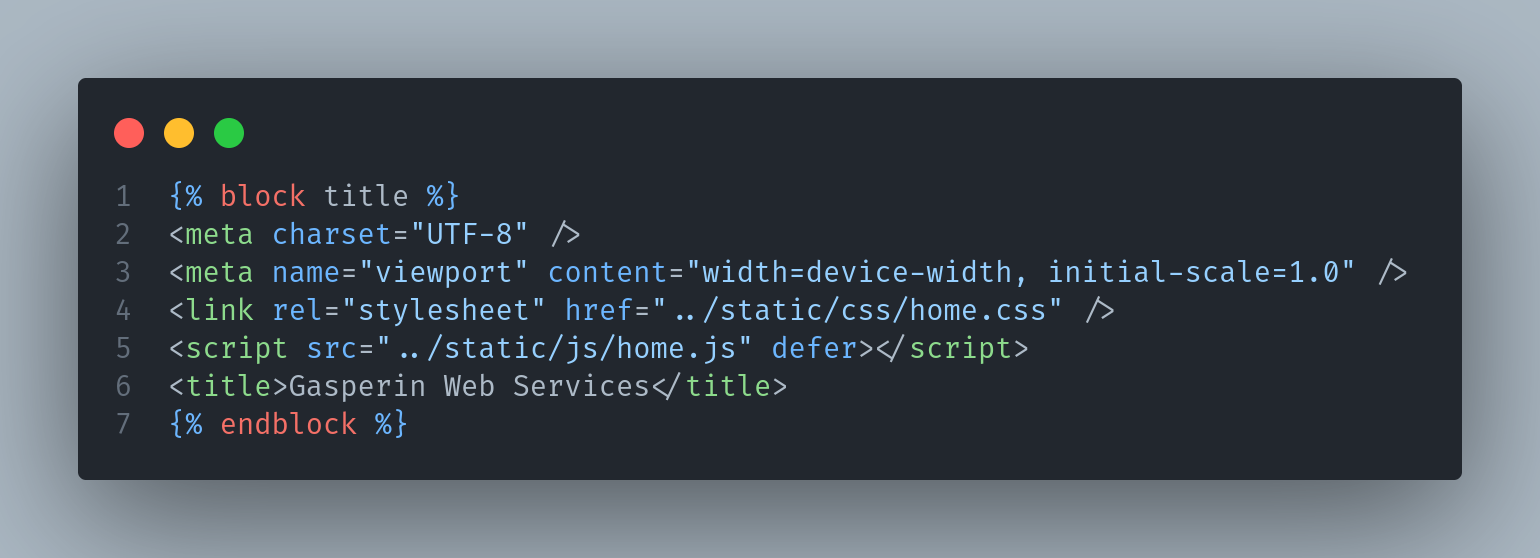
\includegraphics[width=0.30\textwidth]{title-block.png}
        \end{center}
      \end{figure}

      Enquanto o segundo se refere ao conteúdo da página, que estará localizado abaixo do \emph{header} incluso em \emph{layout.html}. Ademais, diversos layouts fazer o uso da linguagem \emph{Jinja2} para mostrar informações de forma dinâmica ao usuário. Por exemplo, o código a seguir cria um elemento \emph{user--card} para cada user passado ao template.

      \begin{figure}[h]
        \begin{center}
          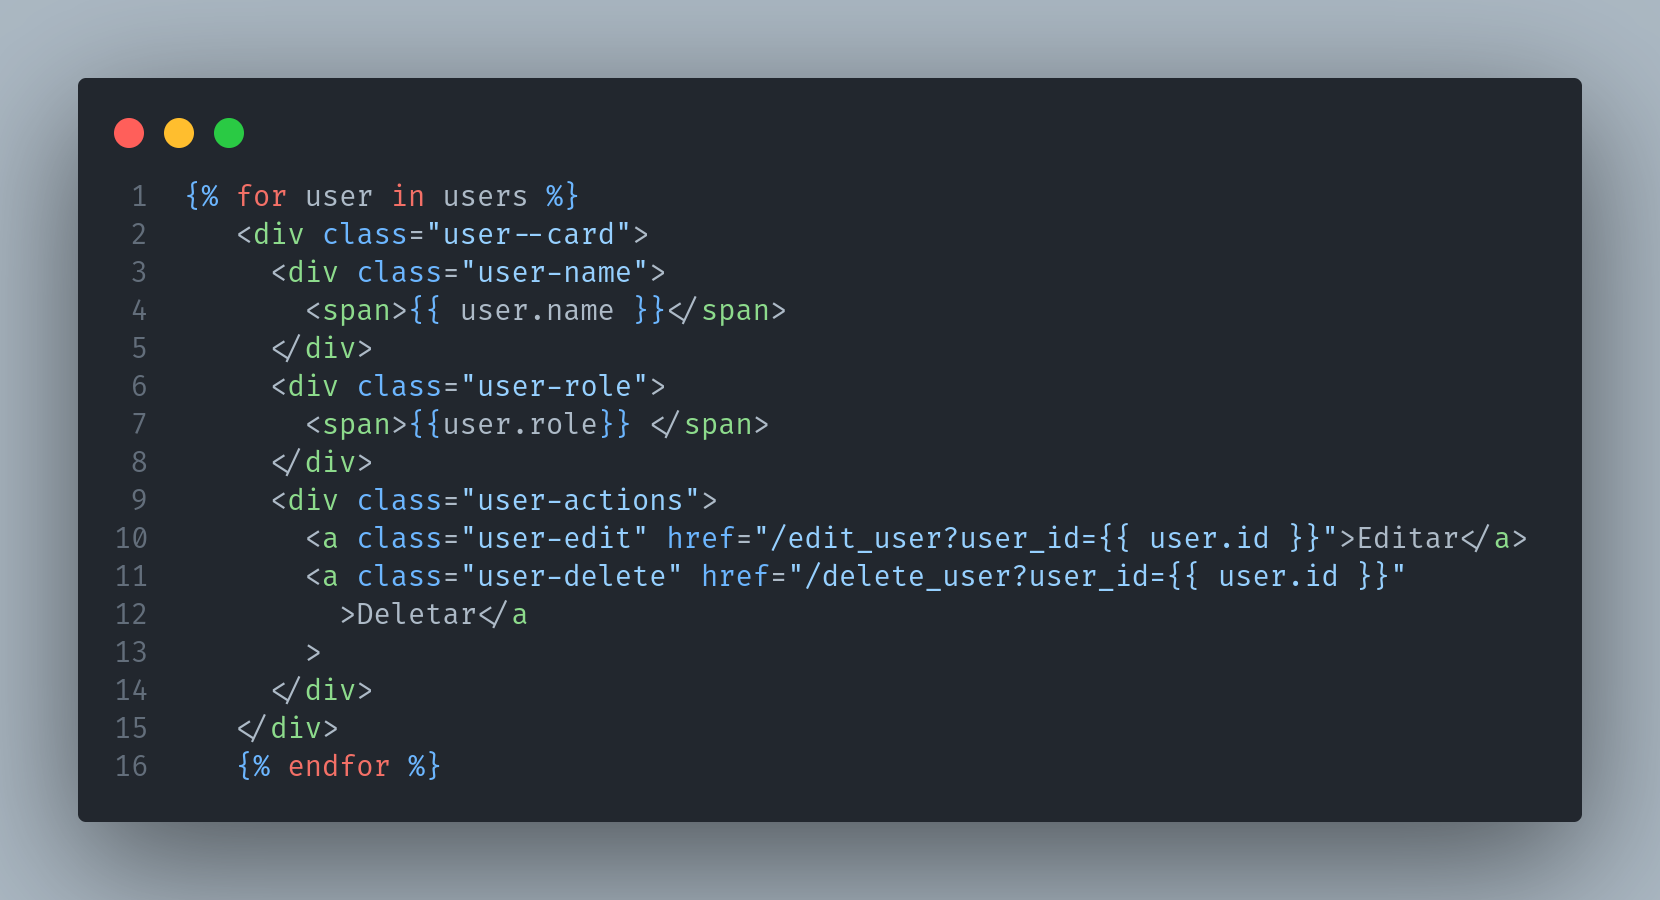
\includegraphics[width=0.30\textwidth]{user-card.png}
        \end{center}
      \end{figure}



\subsubsection{Controllers}
Falar das porcarias dos controllers
\subsubsection{db}
\subsubsection{ESP32}
\subsubsection{ESP32}
O ESP32, integrado neste projeto, desempenha um papel crucial na coleta de dados ambientais e no controle de dispositivos periféricos. Este microcontrolador Wi-Fi e Bluetooth é central para a funcionalidade do sistema, permitindo a comunicação com a Internet e interação com sensores e atuadores.

\paragraph{Conexão Wi-Fi e MQTT}
O ESP32 se conecta à rede Wi-Fi Wokwi-GUEST usando a interface network.WLAN do MicroPython. Após a conexão bem-sucedida, ele se conecta ao servidor MQTT hospedado em mqtt-dashboard.com. Isso facilita a troca de dados entre o dispositivo e outros serviços na nuvem.

\paragraph{Sensores e Atuadores}
\begin{itemize}
\item $Sensor DHT22$: Monitora temperatura e umidade ambiente. O sensor é configurado usando a biblioteca dht e fornece leituras precisas através do método sensor.measure()
\item $Botões de Entrada e Saída$: Gerenciam o controle de fluxo de pessoas com os botões conectados aos pinos 25 e 26. A cada pressionamento, o sistema atualiza o número de pessoas e aciona o servo motor.
\item $Servo Motores$: Controlados pelos pinos 22 (porta) e 27 (janela), ajustam a abertura da porta e da janela com base na quantidade de pessoas e nas condições climáticas.
\end{itemize}
\paragraph{Comunicação MQTT}
Utiliza o cliente MQTT para enviar e receber mensagens do tópico cz/enviar e cz/degar. O método client.publish() envia dados de temperatura, número de pessoas e estado dos botões para o servidor MQTT, enquanto client.subscribe() recebe comandos para controlar o ar-condicionado e a janela.

\paragraph{Monitoramento de Conexão}
A função check\_connection() verifica periodicamente a conexão com o servidor MQTT, reconectando-se automaticamente em caso de interrupções.
\subsubsection{static}
\begin{figure}[h]



  \begin{center}
    
\includegraphics[width=0.30\textwidth]{despair.jpg}
  \end{center}
\end{figure}


\section{Resultados}
\label{sec:results}
% Present the results of the project. This could include screenshots, performance metrics, or other relevant outcomes. Discuss any challenges faced and how they were overcome.
\subsection{Evolução da Aplicação}
As etapas de evolução pelas quais o projeto passou até chegar ao seu estado atual podem ser divididas em 4 principais:
\begin{itemize}
  \item Inicialização dos recursos de hardware
  \item Inicialização da comunicação entre hardware e software
  \item Aplicação do $back$$-$$end$ da aplicação utilizando um banco de dados $MySQL$
  \item Optimização da aplicação
\end{itemize}

\subsection{Inicialização dos recursos de hardware}
Inciando o projeto não utilizamos nenhum recurso de software. No lugar, começamos apenas implementando o hardware.

\subsection{Web}

Ao longo do desenvolvimento do projeto, realizamos várias melhorias para aprimorar a interação do usuário e tornar a aplicação mais dinâmica e intuitiva.

\subsubsection{Tela de Início}

Antes: A tela de início era simples, com poucas opções de navegação e informações básicas.
\begin{figure}[h]
  \begin{center}
    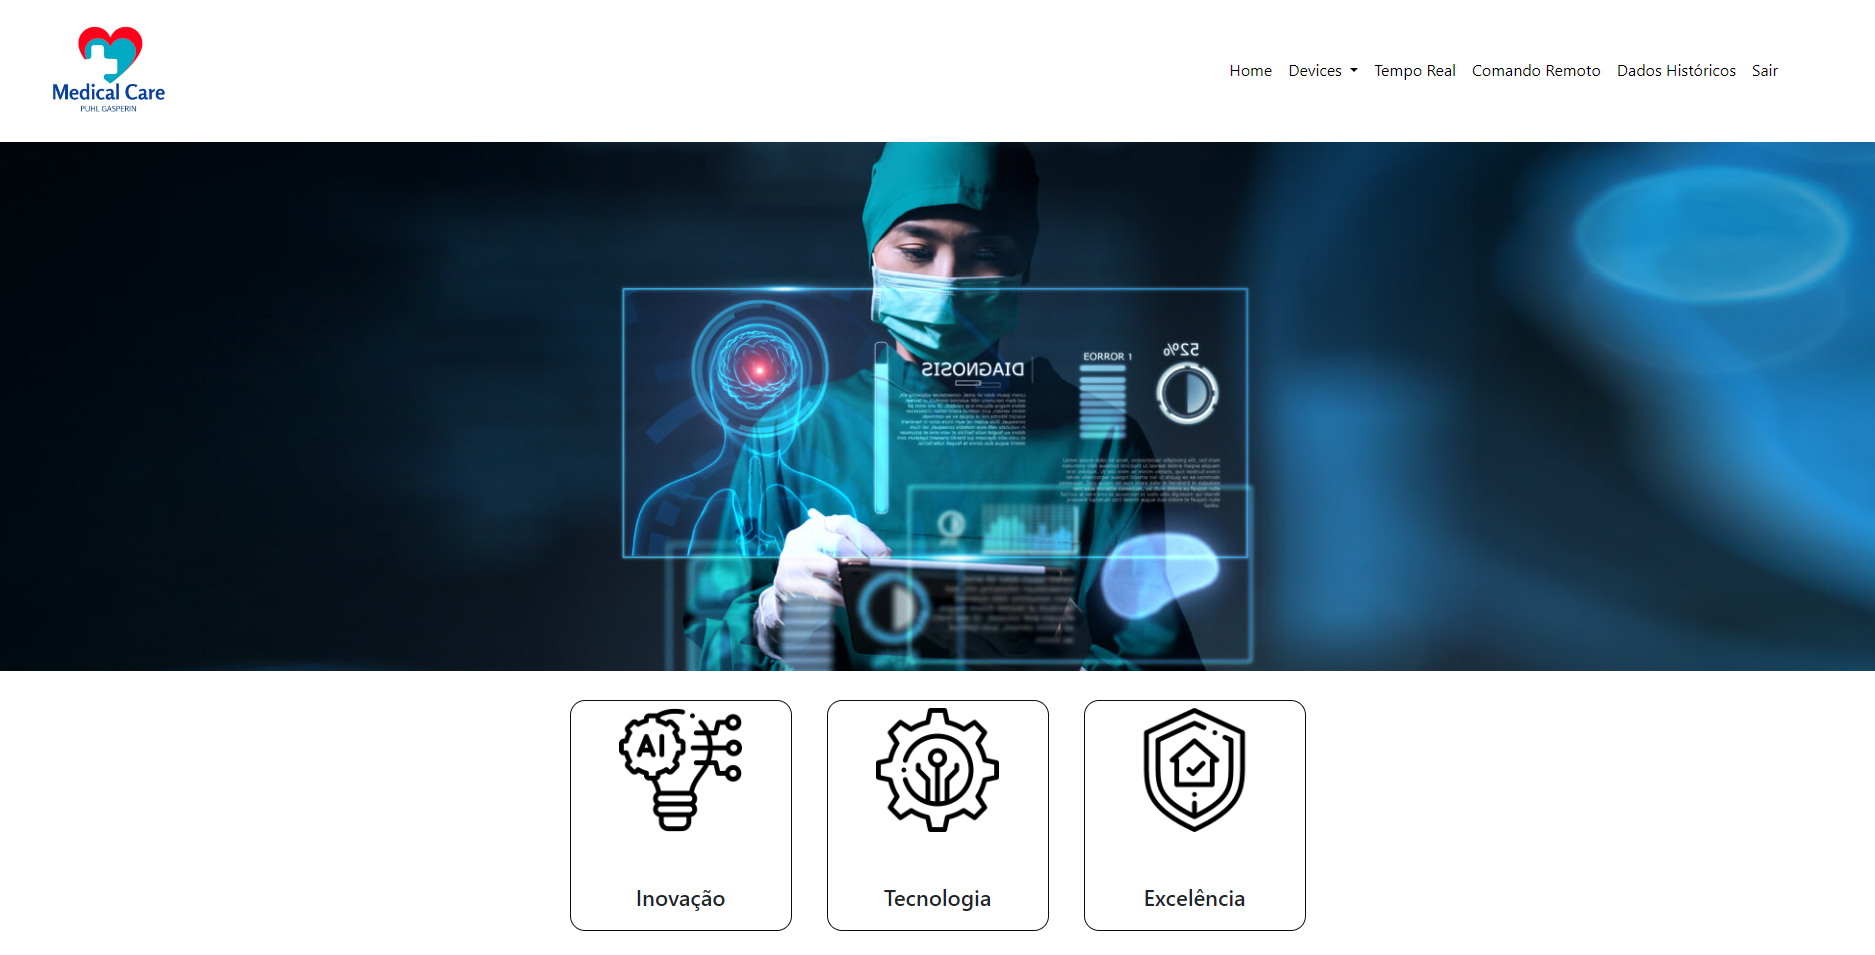
\includegraphics[width=0.5\textwidth]{home_antiga.png}
  \end{center}
\end{figure}

Depois: Incrementamos a tela de início com mais informações relevantes, uma interface mais intuitiva, clara e facil de se encontrar.
\begin{figure}[h]
  \begin{center}
    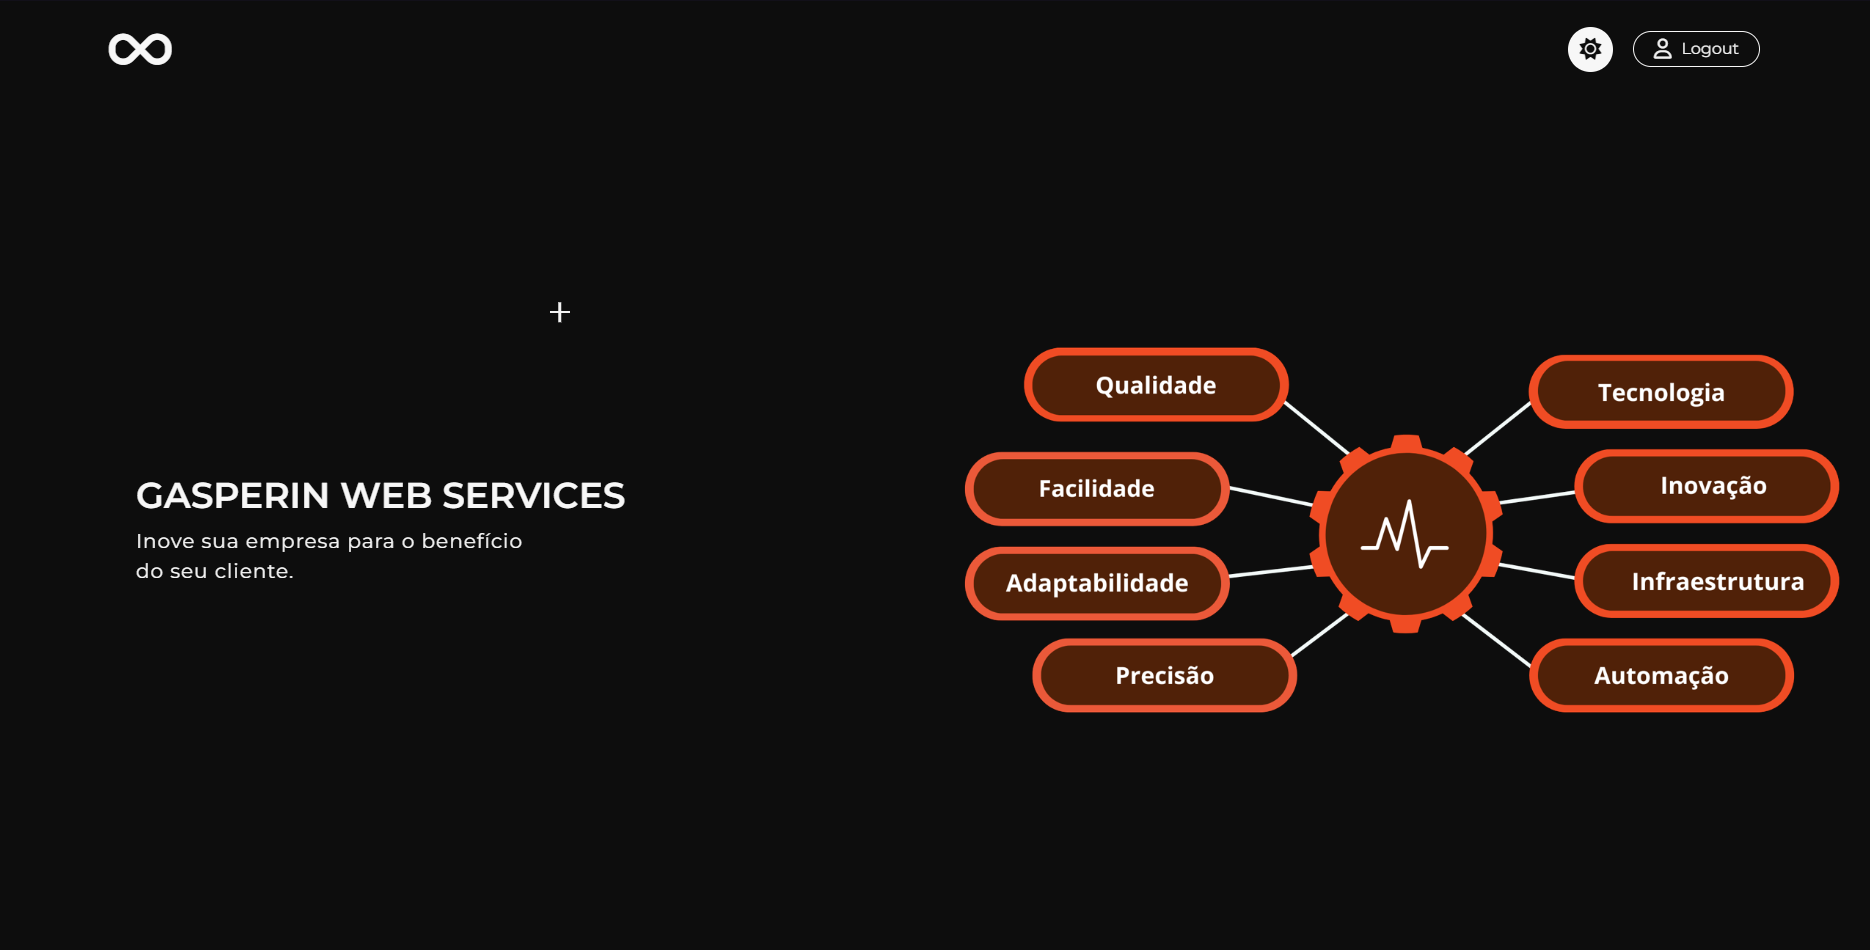
\includegraphics[width=0.5\textwidth]{home_principal.png}
  \end{center}
\end{figure}
\subsubsection{Opções de Administração}

Antes: As opções de administração eram limitadas e pouco intuitivas, com menus básicos que não ofereciam muitas funcionalidades avançadas. A falta de recursos interativos e a interface simplificada dificultavam a gestão eficiente do sistema. Isso impactava diretamente na capacidade de análise detalhada dos dados e na tomada de decisões informadas. Além disso, a ausência de gráficos detalhados e relatórios precisos limitava a compreensão completa do desempenho do sistema. Com a reformulação, procuramos criar um ambiente administrativo mais intuitivo e eficaz. Introduzimos um painel de controle completo com gráficos interativos que proporcionam uma visualização clara e em tempo real dos dados, facilitando a análise e o monitoramento contínuo. Essas mudanças visam não apenas melhorar a usabilidade, mas também aumentar a eficiência operacional e a capacidade de resposta às demandas dos usuários
\begin{figure}[h]
  \begin{center}
    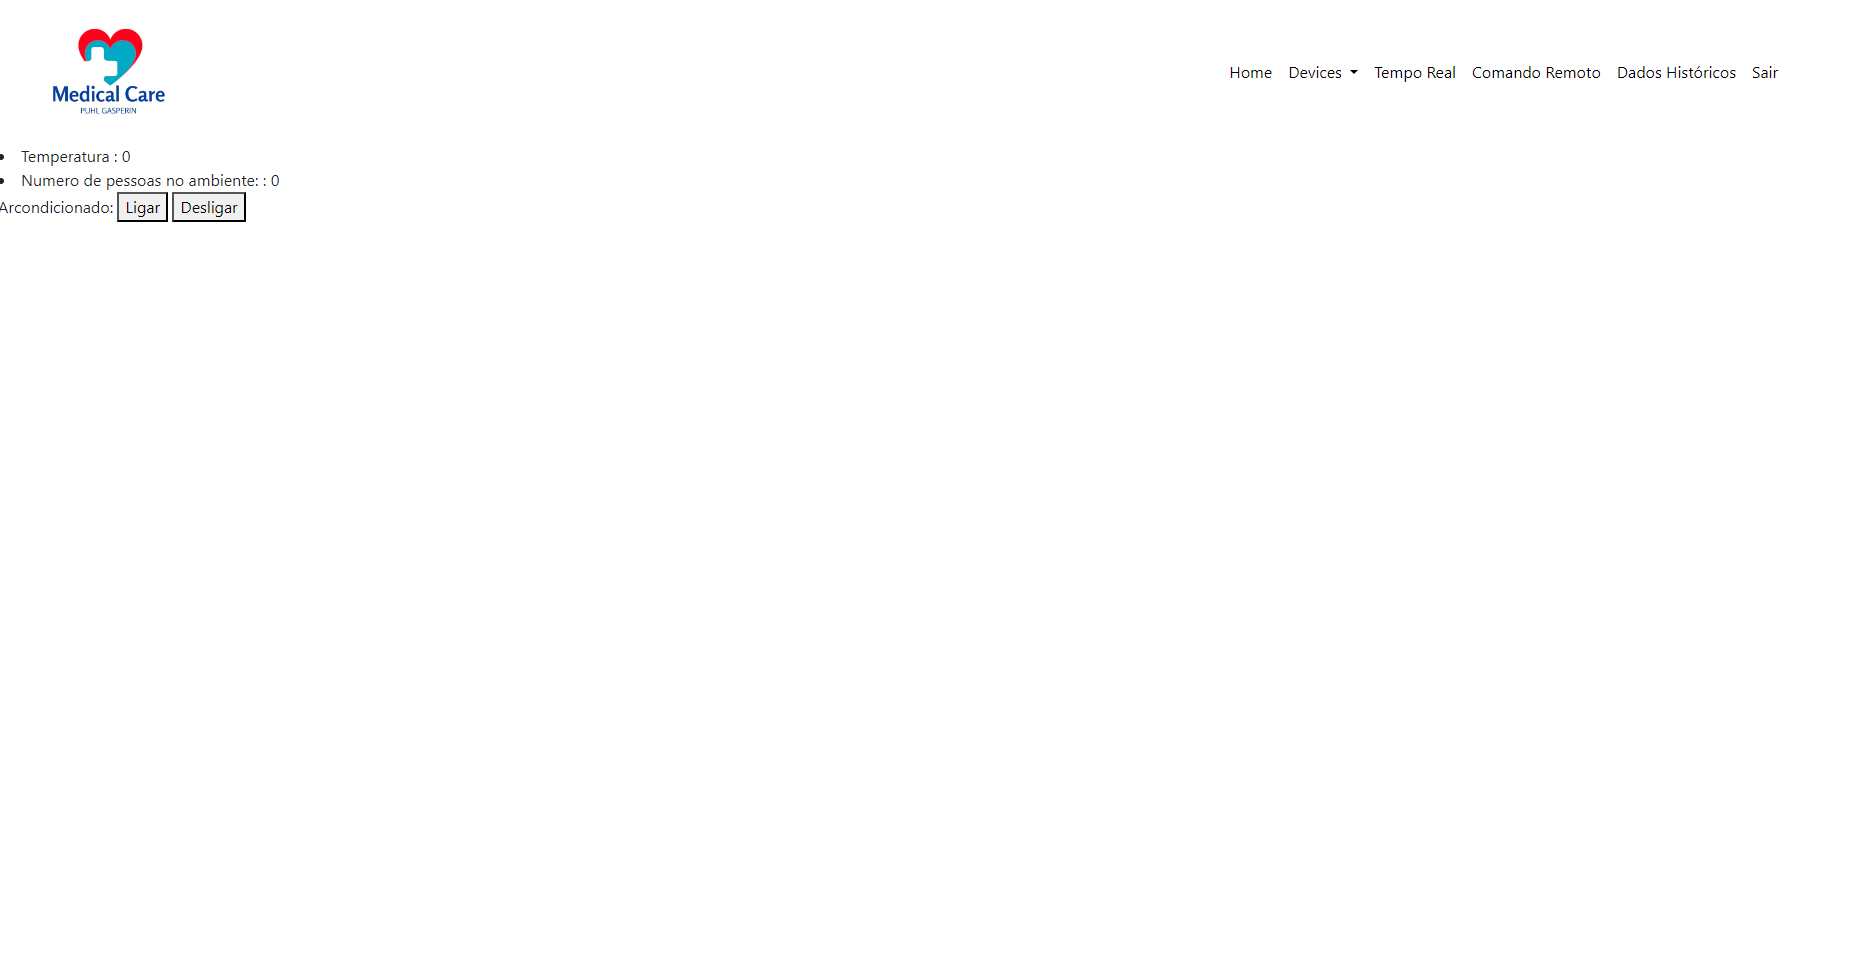
\includegraphics[width=0.5\textwidth]{tempo_real_antiga.png}
  \end{center}
\end{figure}




Depois: Reformulamos as opções de administração, criando um painel mais intuitivo e fácil de usar. Adicionamos novos recursos e opções para facilitar a gestão do sistema, incluindo gráficos interativos e relatórios detalhados.
\begin{figure}[h]
  \begin{center}
    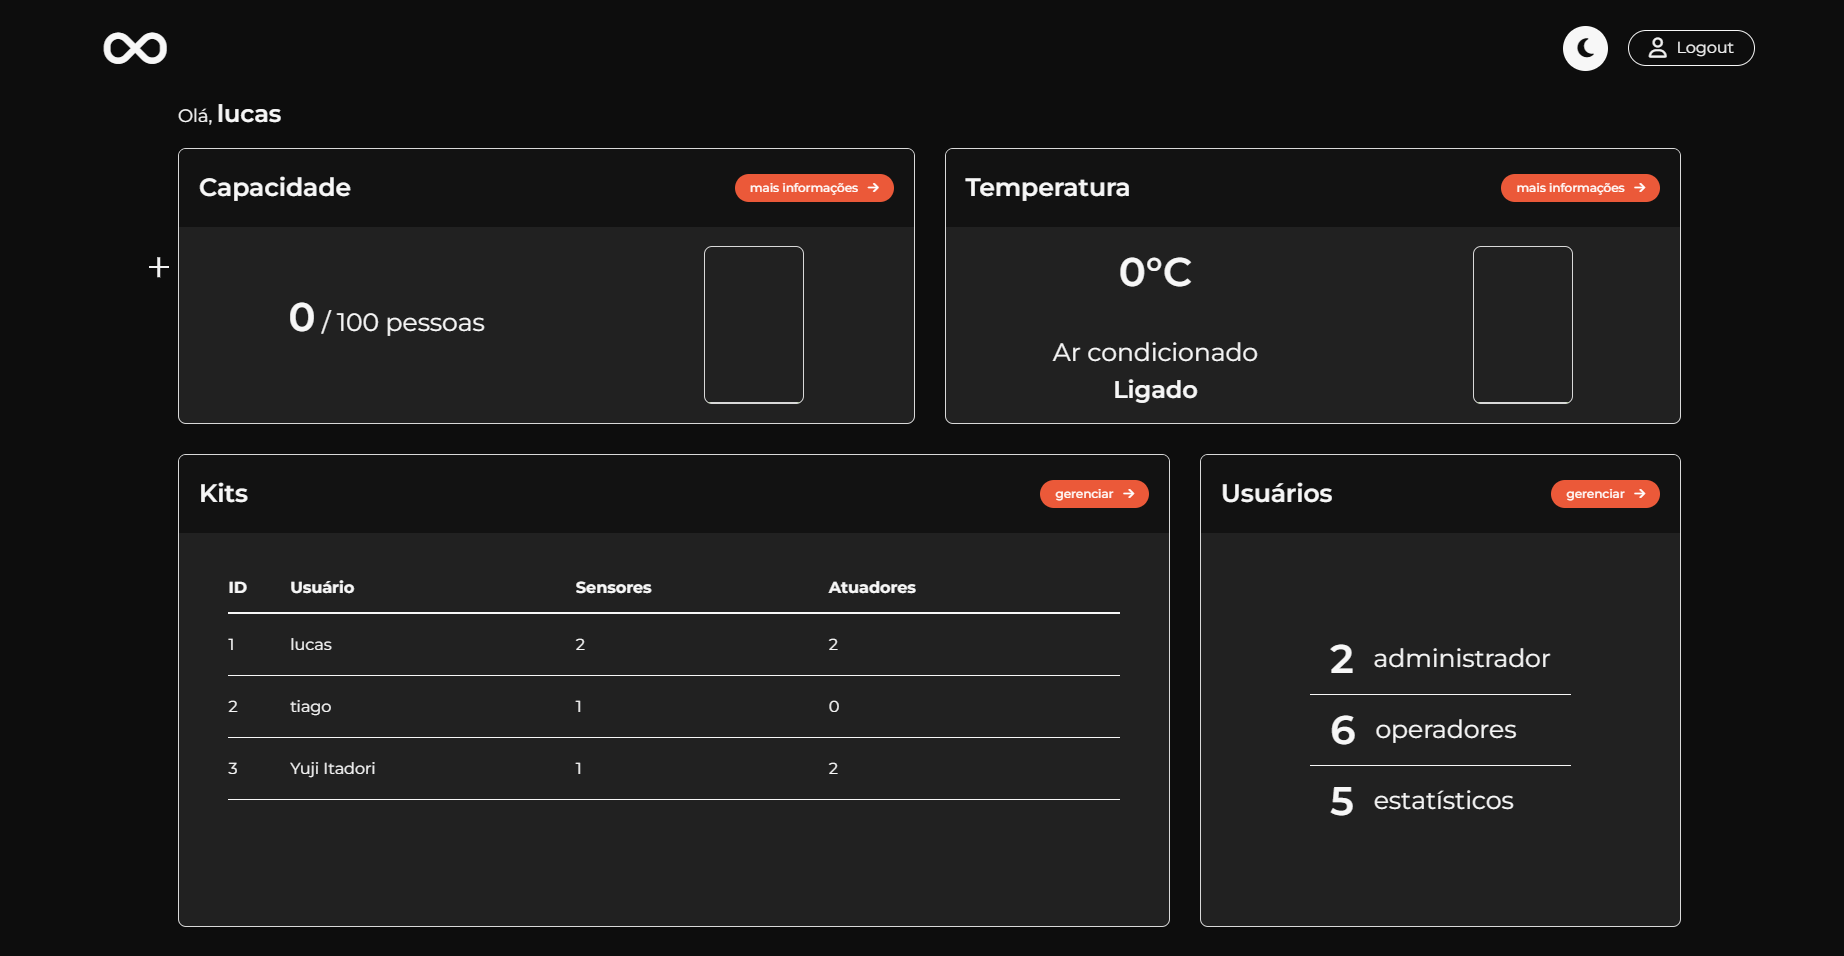
\includegraphics[width=0.5\textwidth]{tempo_real_novo.png}
  \end{center}
\end{figure}


\subsubsection{Nome do projeto}

Antes: O projeto era chamado de Medical Care Puhl Gasperin, um nome que poderia sugerir uma associação direta com serviços médicos e hospitalares.

Depois: Alteramos o nome para Gasperin Web Services para refletir mais claramente nosso objetivo de fornecer uma solução tecnológica para hospitais, sem implicar envolvimento direto com a prática médica. Esse novo nome comunica melhor nosso foco em serviços tecnológicos e gerenciamento de ambientes hospitalares.


\subsubsection{Modos de Exibição}

Implementamos a opção de modos de exibição dark e light, permitindo que o usuário escolha a interface que melhor se adapta às suas preferências. Essa funcionalidade pode ser facilmente ajustada a qualquer momento, proporcionando maior flexibilidade e conforto visual ao usuário.
\subsubsection{Vai tomar no cu}
\subsubsection{Preciso de umas imagens}
IMAGEM IMAGEM IMGAGEM

\begin{figure}[h]

  \begin{center}
    
\includegraphics[width=0.30\textwidth]{help.jpeg}
  \end{center}
\end{figure}

\subsection{Banco de dados}
\subsubsection{Flask Login}

\section{Discussão}
\label{sec:discussion}
% Analyze the results and their implications. Discuss what went well, what could be improved, and any lessons learned during the development process.
  O desenvolvimento da aplicação web para o monitoramento do fluxo de pessoas em postos de saúde representa um avanço significativo na gestão e eficiência desses ambientes. A possibilidade de controlar a abertura e fechamento de portas conforme a demanda de pacientes permite uma organização mais dinâmica e adaptável às necessidades reais, melhorando a experiência dos usuários e otimizando os recursos humanos e materiais disponíveis. Além disso, a integração de sistemas para abertura e fechamento de janelas e controle do ar condicionado conforme a temperatura ambiente não só proporciona um ambiente mais confortável para pacientes e profissionais de saúde, mas também promove a eficiência energética, reduzindo os custos operacionais dos estabelecimentos.

  Os resultados preliminares indicam uma melhoria na fluidez do atendimento e uma redução no tempo de espera dos pacientes. A capacidade de monitoramento em tempo real permite uma resposta rápida a situações de alta demanda, evitando aglomerações e garantindo um atendimento mais organizado e seguro, especialmente em tempos de pandemia. No entanto, algumas falhas foram observadas durante o processo de implementação. Problemas de conectividade foram identificados como pontos críticos que necessitam de soluções para garantir a confiabilidade do sistema. Como solução, deve-se investir em equipamentos duradouros e de qualidade, a fim de providenciar um funcionamento constante e duradouro.

  As implicações futuras dessa tecnologia são promissoras. A possibilidade de criar um aplicativo móvel que não apenas mostre os dados de ocupação em tempo real, mas também direcione os pacientes para o posto de saúde mais adequado conforme a demanda atual, pode revolucionar o acesso aos serviços de saúde. Essa funcionalidade reduziria ainda mais os tempos de espera e distribuiria melhor os pacientes entre as diversas unidades, evitando sobrecargas em determinados locais e subutilização em outros. Ademais, a análise dos dados coletados pode fornecer $insights$ valiosos sobre padrões de utilização dos serviços de saúde, permitindo uma melhor gestão e planejamento. 

  Entretanto, a implementação desse sistema requer a consideração de diversos fatores. Visto que existem diversos sistemas já em produção dentro dos postos de saúde públicos, é fundamental assegurar a compatibilidade do novo sistema com estes já existentes, promovendo uma integração eficiente e sem falhas. Investimentos em infraestrutura tecnológica e treinamento de pessoal são igualmente essenciais para o sucesso do projeto a longo prazo.

  Em resumo, a aplicação web desenvolvida apresenta um potencial significativo para melhorar a gestão dos postos de saúde, proporcionando um atendimento mais eficiente e confortável para os pacientes. As falhas identificadas são superáveis com investimentos adequados em tecnologia e infraestrutura. As futuras expansões, incluindo o desenvolvimento de um aplicativo móvel e a análise de dados para aprimoramento contínuo dos serviços, delineiam um caminho promissor para a modernização e otimização do sistema de saúde pública.

  Ademais, a proposta da empresa $Gasperin$ $Web$ $Services$ abre portas para atender diversos outros clientes posteriormente, não apenas gerenciando o controle automatizado do fluxo de pessoas e clima ambiente, mas também outros meios de inovação via serviços web. Através desse projeto, a $GWS$ demonstra sua competência em áreas-chave que são altamente relevantes para uma variedade de outros setores e mercados globais.

\section{Conclusão}
\label{sec:conclusion}
% Summarize the key points of the document. Reiterate the significance of the project and its contributions. Suggest possible future work or improvements.

  Em resumo, a aplicação web desenvolvida apresenta um potencial significativo para melhorar a gestão dos postos de saúde, proporcionando um atendimento mais eficiente e confortável para os pacientes. As falhas identificadas são superáveis com investimentos adequados em tecnologia e infraestrutura. As futuras expansões, incluindo o desenvolvimento de um aplicativo móvel e a análise de dados para aprimoramento contínuo dos serviços, delineiam um caminho promissor para a modernização e otimização do sistema de saúde pública.

  O projeto aqui descrito demonstra a viabilidade e a utilidade de soluções tecnológicas avançadas na gestão de serviços de saúde. Com a capacidade de monitorar e ajustar o fluxo de pacientes em tempo real, abre-se uma nova era de eficiência operacional e qualidade no atendimento. A implementação de sistemas automatizados para controle de portas, janelas e climatização não só melhora o conforto dos usuários como também contribui para a sustentabilidade dos recursos energéticos. O próximo passo envolve a ampliação das funcionalidades da aplicação, incluindo a criação de um aplicativo que possa informar os usuários sobre a lotação dos postos de saúde e direcioná-los de forma inteligente para as unidades mais adequadas.

  A incorporação dessas tecnologias emergentes no dia a dia dos serviços de saúde pode levar a uma transformação significativa, onde a gestão de fluxo e a alocação de recursos se tornem mais eficazes e responsivas. Para alcançar esse futuro, é essencial um compromisso contínuo com a inovação, o investimento em tecnologia e a formação de profissionais capacitados para lidar com esses novos sistemas. Dessa forma, poderemos garantir que os avanços tecnológicos se traduzam em benefícios reais e duradouros para a sociedade.






\section{Referencias}
\label{sec:references}
% List all references used in the preparation of the document, including books, articles, and online resources.
\bibliographystyle{IEEEtran}
\bibliography{references}

\end{document}